\section{Zielsetzung}
Ziel ist es, aus den Wellenlängen $\lambda$ der Spektrallinien verschiedener Alkalimetalle auf die jeweilige Abschirmkonstante $\sigma$ zu schließen.


\section{Theorie}
\label{sec:Theorie}

Der Vorteil der Verwendung von Alkali-Metallen besteht darin, dass eine Ein-Elektronen-Näherung durchgeführt werden kann. Diese Näherung ist möglich, da Alkali-Metalle ein oder mehrere abgeschlossene Elektronenschalen aufweisen mit einem einzelnen Elektron auf der äußersten Schale. Jedoch muss der Unterschied zum Wasserstoffatom mit der Abschirmzahl $\sigma$, die die Abschwächung des Coulombfeldes durch die abgeschlossenen Elektronenschalen beschreibt, korrigiert werden.
\subsection{Berechnung der Strahlungsenergie}
Ausgehend von der stationären Schrödingergleichung
\begin{align}
  H \coloneqq \sum_{i}^N \frac{P_\textrm{i}^2}{2m_\textrm{i} + U} \;,
  \label{eq:SG}
\end{align}
wird zuerst das Potential eines Wasserstoffatoms unter Berücksichtigung der Abschirmzahl $\sigma$ ergänzt, somit ergibt sich
\begin{align}
  H = \frac{P_\textrm{i}^2}{2m_\textrm{i}} - \frac{(z-\sigma)e_0^2}{4\pi\epsilon_0 r} \;.
  \label{eq:SG_mit_sigma}
\end{align}
Aufgrund der Zentralsymmetrie bietet sich die Benutzung von Kugelkoordinaten an. Demzufolge wird der Laplace-Operator in einen Radial- und in einen Winkelanteil zerlegt. Mit Hilfe des quantenmechanischen Drehimpulses lässt sich der Ausdruck zusammenfassen zu
\begin{align}
  H = -\frac{\hbar^2}{2m_0} \frac{1}{r} \frac{\partial^2}{\partial r^2}r + \frac{\hbar^2}{2m_0}l(l+1) \frac{1}{r^2} - \frac{(z-\sigma)e_0^2}{4\pi\epsilon_0} \frac{1}{r} \;.
  \label{eq:SG_mit_Drehimpuls}
\end{align}
Durch die erlaubte Vertauschung des Drehimpulses $L$ mit dem Hamilton-Operator $H$, besitzt der Drehimpuls die gleichen Eigenfunktionen
\begin{align}
  L^2\psi = w^2 \psi \;.
  \label{eq:Eigenfkt_Drehimpuls}
\end{align}
Die Eigenfunktion dieser Differenzialgleichung ist die Kugelflächenfunktion $Y_\textrm{l}(\vartheta,\varphi)$.  Der Laufindex $l$ bezeichnet die Bahndrehimpulsquantenzahl.
Zu der Hauptquantenzahl $n$ besteht der folgende Zusammenhang
\begin{align}
  l_\textrm{max} = n - 1 \; .
\end{align}
Diese $l$-Abhängigkeit zeigt sich auch in den Energieeigenwerten, wenn die Relativitätstheorie einbezogen wird. Dieser Einfluss der Relativitätstheorie wird nur als Störungsfaktor in dem Hamilton-Operator berücksichtigt. Zu diesem Zweck wird der Hamilton-Operator in erster Ordnung verwendet. Somit ergibt sich für die Energieeigenwerte
\begin{align}
  E_\textrm{rel} = -R_\textrm{\infty} \left\{ \frac{(z-\sigma)^2}{n^2} + \alpha^2\frac{(z-\sigma)^4}{n^3} \left( \frac{2}{2l+1}-\frac{3}{4n} \right) \right\} \;\;
  \text{mit}\;
  \alpha \coloneqq \frac{e_0^2}{2hc\epsilon_0} \;.
  \label{eq:Energieeigenwerte}
\end{align}
Durch die zweite Quantenzahl werden die $n$ Energieniveaus in $l$ Unterniveaus unterteilt.\\
Für eine höhere Genauigkeit der Gleichung $\ref{eq:SG_mit_Drehimpuls}$, muss der Spin des Elektrons einbezogen werden. Dieses führt zu der dritten Quantenzahl $s$ die jedoch nur den Wert $s= \pm\frac{1}{2}$ annimmt. Aufgrund des Spins treten magnetische Momenten auf, weshalb Wechselwirkungen auftreten, die als Spin-Bahn-Kopplung bezeichnet werden.
Die Kopplung hat zufolge, dass sich der jeweilige Spin bzw. Drehimpuls des Elektrons vektoriell zu einem Gesamtdrehimpuls $\vec{J}$ zusammensetzt. Aus den Eigenwertgleichungen des $S$ und  des $L$ Operators ergibt sich der Hamiltonoperator
\begin{align}
  H_\textrm{SpB} = \frac{1}{2m_0^2c^2} \frac{1}{r} \frac{\text{d}U}{\text{d}r} S\cdot L - \frac{e_0 \hbar^2}{8m_0^2c^2}\text{div}\frac{(z-\sigma)e_0}{4\pi \epsilon_0} \frac{\vec{r}}{r^3} \; .
  \label{eq:Hamiltonoperator}
\end{align}
Aus der Eigenwertgleichung von $S\cdot L$ und dem berechneten Coulomb-Potential ergibt sich die Gleichung für die Energieeigenwerte
\begin{align}
  E_\textrm{n,j} = -R_\infty \left\{ \frac{(z-\sigma)^2}{n^2} + \alpha^2 \frac{(z-\sigma)^4}{n^3} \left( \frac{1}{j+\frac{1}{2}} - \frac{3}{4n} \right) \right\}
\end{align}
unter Berücksichtigung, dass $j$ nur die Werte $l + \frac{1}{2}$ und $l - \frac{1}{2}$ annehmen kann.
\subsection{Auswahlregeln für Quantenübergänge}
Für die Differenz der Hauptquantenzahl $\Delta  n$ von einem Energieniveau zum anderen, existieren keine Einschränkungen, wobei Übergänge mit einer großen Differenz zunehmend unwahrscheinlicher werden.\\
Da Energieniveaus mit gleichem $n$ und $l$, aber unterschiedlichem j, diejenigen Energieniveaus sind, die am dichtesten zusammen liegen, werden sie als Dublett-Struktur bezeichnet. Die Dublett-Struktur ist in Abb. \ref{fig:Energieniveaus} dargestellt.\\
\begin{figure}
  \centering
  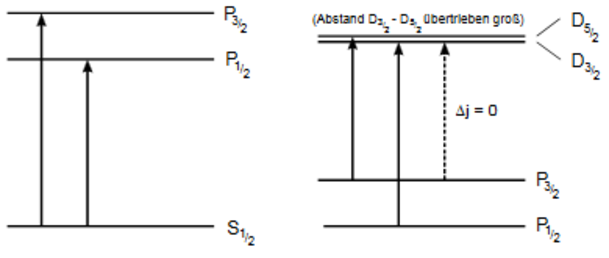
\includegraphics{ressources/Energieniveaus.pdf}
  \caption{Darstellung verschiedener Energieniveaus \cite{skript}.}
  \label{fig:Energieniveaus}
\end{figure}

Zudem gibt es eine Einschränkung der Differenz der Quantenzahl $\Delta l$. Energieniveauübergänge ohne Änderung des Bahndrehimpulses $\Delta l= 0$ sind nicht möglich. Für die "erlaubten" Übergänge gilt $\Delta l = \pm 1$.\\
Übergänge, bei denen keine Änderung der Quantenzahl $j$ auftritt, sind zum einen sehr unwahrscheinlich und zum anderen, wenn sie auftreten, schlecht zu beobachten, da beim Übergang kein Photon emittiert wird.

\subsection{Die Abschirmkonstanten}
Bei der Berechnung der Energieeigenwerte müssen die beiden Abschirmkonstanten $\sigma_1 , \sigma_2$ berücksichtigt werden. Die erste Abschirmkonstante $\sigma_1$ beschreibt die Abschirmung des vom Kern verursachten Coulomb-Feldes von den Elektronen. Die Kern-nahen Elektronen, die sogenannten Rumpfelektronen, beeinflussen dieses Feld deutlich stärker als Elektronen auf äußeren Schichten. Bei der zweiten Abschirmkonstante $\sigma_2$ wird die Spin-Bahn-Kopplung des beobachteten, äußeren Elektrons berücksichtigt. Dabei wird ermittelt wie groß die Abschirmung der Elektronen auf der Schale des Leuchtelektrons  ist. Somit ist $\sigma_1 \ge \sigma_2$.
Weiter ergibt sich die Gleichung für die Energieeigenwerte mit den Abschirmkonstanten zu
\begin{align}
  E_\textrm{n,j} = - R_\infty \left\{ \frac{(z-\sigma_1)^2}{n^2} + \alpha^2\frac{(z-\sigma_2)^2}{n^3} \left( \frac{1}{j+\frac{1}{2}} - \frac{3}{4n} \right) \right\}  \; .
  \label{eq:Energieeigenwerte_mit_Abschirmkonst.}
\end{align}
In diesem Experiment soll die Abschirmkonstante $\sigma_2$ bestimmt werden. Da die Energiedifferenz $\Delta E_\textrm{D}$ in einem Dublett bestimmt wird, ändert sich beim Übergang nur die Quantenzahl $j$. Aus diesem Grund ergibt sich die Energiedifferenz $\Delta E_\textrm{D}$ durch
\begin{align}
  \Delta E_\textrm{D} &= E_\textrm{n,j} - E_\textrm{n,j+1}\\
   &= \frac{R_\infty \alpha^2}{n^3}(z-\sigma_2)^4 \frac{1}{l(l+1)} \\
  \Leftrightarrow \; \; \sigma_2 &= z - \sqrt[4]{\frac{\Delta E_\textrm{D}(l(l+1))n^3}{R_\infty \alpha^2}} \;.
  \label{eq:sigma2}
\end{align}

Die in Gleichung \ref{eq:sigma2} benötigte Energiedifferenz $\Delta E_\textrm{D}$ wird durch die ermittelte Wellenlänge $\lambda$ mit
\begin{align}
  \Delta E_\textrm{D} = hc\left(\frac{1}{\lambda} - \frac{1}{\lambda'} \right) \approx h c\frac{\Delta\lambda}{\lambda^2}
  \label{eq:E_D}
\end{align}
berechnet.
\subsection{Das Beugungsgitter}
Das Beugungsgitter besteht aus einer großen Anzahl parallel ausgerichteter Spalten. Bestrahlt man dieses mit einem Lichtstrahl, wird dieser teilweise unter einem bestimmten Winkel reflektiert. Wie groß der Beugungswinkel ist, hängt von der Wellenlänge $\lambda$ des einfallenden Lichtes ab. Somit kann durch den Reflexionswinkel $ 	\varphi$ auf die Wellenlänge $\lambda$ geschlossen werden, wenn die Spaltenanzahl $p$, die Spaltenbreite $b$ und die Gitterkonstante $g$ bekannt sind. Um diese zu berechnen sei die Amplitude der Welle
\begin{align}
  E(z,t) = E_0 \exp{i\left(\omega t - 2\pi \frac{z}{\lambda}\right)} \; .
\end{align}
Da der Teilchenstrahl zum einen nach dem Austritt eines Spaltes mit der Breit $b$ mit sich "selbst" interferiert, ist die Intensität gegeben durch
\begin{align}
  I_\textrm{b}( 	\varphi) = E_0^2 b^2 \left( \frac{\lambda}{\pi b \sin{ 	\varphi}} \right) \sin{ \left( \frac{\pi b \sin{\varphi}}{\lambda}\right)}^2
\end{align}
und zum anderen mit den Lichtstrahlen aus den anderen Spalten interferiert ergibt, sich für die Gesamtintensität
\begin{align}
  I_\textrm{g}(\varphi) = |E_\textrm{g}(\varphi)|^2 I_\textrm{b}(\varphi) \;.
\end{align}
Um $E_\textrm{g}(\varphi)$ zu bestimmen, wird der Phasenunterschied $\delta$ einer Welle zwischen zwei Spaltausgängen betrachtet. Hier für ergibt sich nach Abb. $\ref{fig:Beugung}$
\begin{align}
  \delta = \frac{2 \pi g \sin{(\varphi)}}{\lambda} \; .
\end{align}

\begin{figure}
  \centering
  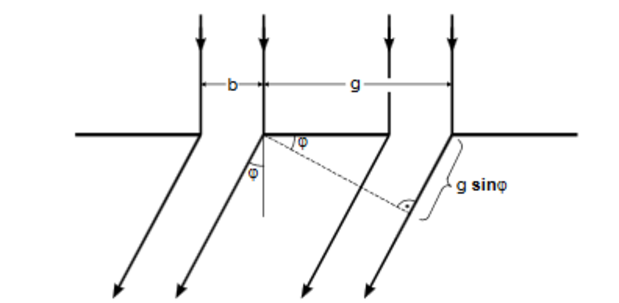
\includegraphics{ressources/Beugung.pdf}
  \caption{Beugung einer ebenen Welle an regelmäßig angeordneten Spaltöffnungen der Breite $b$ \cite{skript}.}
  \label{fig:Beugung}
\end{figure}

Für $p$ Spalten setzt sich die Amplitude $E_\textrm{g}(\varphi)$ aus $p$ überlagerten Teilwellen zusammen. Somit gilt die folgende Beziehung zwischen der Amplitude und der Phasenverschiebung
\begin{align}
  |E_\textrm{g}(\varphi)|^2 = \frac{\sin({p \frac{\delta}{2}}^2)}{\sin({\frac{\delta}{2}}^2)} \;.
\end{align}
Weiter wird für jedes Gitter individuell der jeweilige Spaltenfaktor
\begin{align}
    s(x) \coloneqq \frac{\sin({x})^2}{x^2} \qquad \qquad \qquad  \text{mit} \; x \coloneqq \pi b \sin({\varphi/\lambda})
\end{align}
und der Gitterfaktor
\begin{align}
  	g(y) \coloneqq \frac{\sin({py}^2)}{\sin({y}^2)} \qquad \qquad \qquad  \text{mit}  \; y \coloneqq \pi g \sin({\varphi/\lambda})
\end{align}
definiert. Aus diesen Größen werden die Hauptmaxima an der Stelle
\begin{align}
  \sin({\varphi}) = k\frac{\lambda}{g}, \qquad \qquad \qquad  k = 0,1,2, ...
  \label{eq:sinphi}
\end{align}
lokalisiert. Wird $p$ entsprechend groß gewählt, wird der Abstand der Minima beliebig klein. Wie in Abb. $\ref{fig:Maxima}$ zu sehen werden dadurch die Maxima beliebig schmal, was zur folge hat, dass im Experiment helle Linien zu erkennen sind.

\begin{figure}
  \centering
  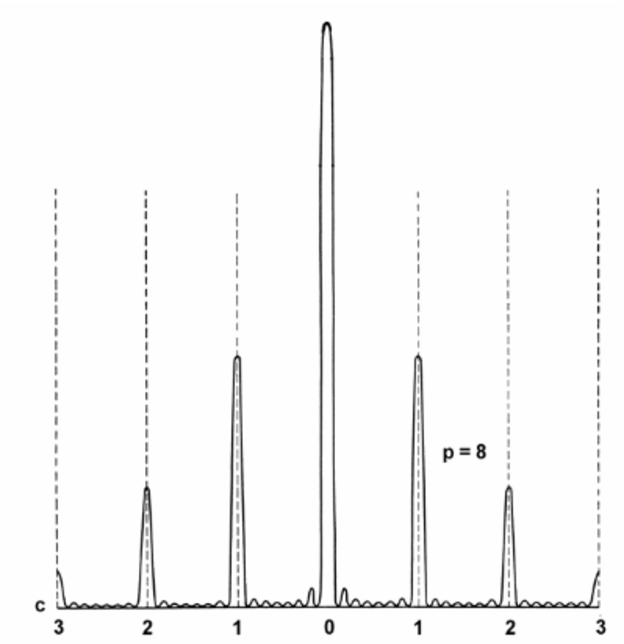
\includegraphics{ressources/Maxima.pdf}
  \caption{Intensitätsverteilung (qualitativ) bei der Beugung durch 8 Spalte \cite{skript}.}
  \label{fig:Maxima}
\end{figure}
